% $  Id: validation.tex  $
% !TEX root = main.tex


%%
\section{Validation}
\label{sec:validation}

To validate the appropriateness of CollabIDE, we define two research questions
\begin{enumerate*}[label=(\arabic*)]
\item improve productivity, and
\item SPL
\end{enumerate*} 
To answer these questions, we conducted an empirical evaluation 
to measure how effective CollabIDE was at reducing overhead problems 
in both Distributed Software Development and Software Product Lines.

%%%%
\subsection{Experiment Design}

\authorcomment[missing]{NC}{Context, Research questions, analysis method, data collection method}

For each research question, we designed one experiment. In each experiment, we asked 
a group of developers to solve programming tasks using either CollabIDE or a 
conventional IDE following a set of instructions that aim to emulate the workflow that is carried out in each development model. The experiments differed in team sizes, the tasks that needed to be completed and the workflow each set of participants had to follow. Two metrics were taken in each experiment, first, the percentage of completion of the total tasks assigned and second, the amount of time in minutes spent performing actions related to version control.

%%%%
\subsubsection{Experiment 1: Software development in a distributed set-up}
The objective of this experiment was to quantify the overhead reduction that can be achieved with CollabIDE in a distributed development project where team members must use version control constantly to always have up to date code. 
For the experiment, groups of developers had to use JavaScript to accomplish their given programming tasks and must also had to use version control periodically so that both team members code remained up to date through the experiment. 


%%%%
\subsubsection{Experiment 2: Product variants development and deployment}
In this second experiment the objective was to also quantify the overhead reduction that can be achieved with CollabIDE within a product line development context where various variants of a product must be maintained.
For the experiment, individual developers had to program in Java or JavaScript depending on the IDE they used to complete their tasks. Additionally, they had to use version control to manage the different product variants that were involved in the programming tasks.


\begin{figure}[htbp]
  \centering
  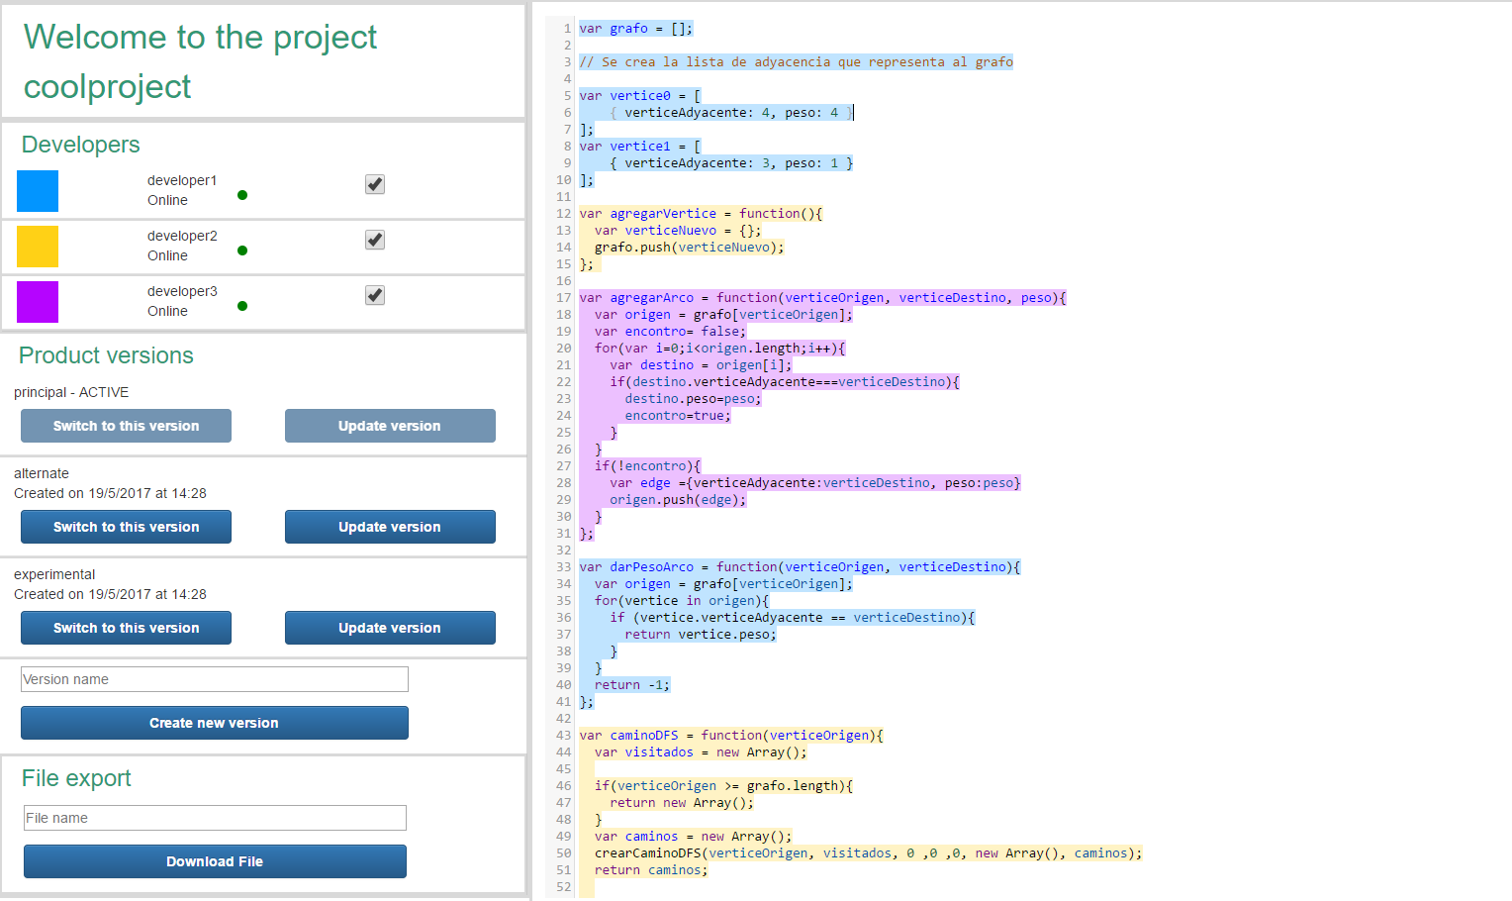
\includegraphics[width=0.7\textwidth]{img/fig1-collabIDEGeneral}
  \caption{CollabIDE tool}
  \label{fig:collabide}
\end{figure}

%%%%
\subsection{Experiment Setup}

Six developers were gathered for the Distributed Software Development experiment, then they were split into groups of two. Two groups would be using CollabIDE and the remaining group would be using Sublime Text in conjunction with git and github. The programming task for this experiment was to implement a set of common graph algorithms using only JavaScript. The participants were given a total of ninety minutes to accomplish this task. Each group was required to obtain their partner’s changes every fifteen minutes using their tools at hand.
In the Software Product Lines experiment, a different group of four developers was gathered. Two of them would be using CollabIDE and the other two would be using Eclipse in conjunction with git and github. In this case, the programming task was to implement a set of data structures with some basic functionality using JavaScript (CollabIDE) or Java (Eclipse). Each data structure also had to be a variant of a given base structure. These participants were also given ninety minutes to complete their task. In order to manage the different product variants, the participants were requested to use version control in each of their IDEs.


\authorcomment[missing]{NC}{Tools, exercise}
	

%%%%
\subsection{Results}

At the end of the experiment, the metrics showed that the developers which used CollabIDE obtained 
a higher completion percentage than those who used the other IDEs. The developers who used 
CollabIDE also spent significantly less time doing actions related to version control than the 
developers that used other IDEs.

%%%%
\subsection{Threads to Validity}
En esta sección discutimos algunos aspectos del experimento que pueden poner en peligro la validez de los resultados. El primero es que la muestra de participantes es muy baja, en el primer experimento tan solo hubo un grupo de control y dos grupos con CollabIDE, del mismo modo en el segundo experimento solo hubo 2 participantes en cada IDE. Cuando las muestras de participantes son bajas, es más fácil caer en el sesgo [11]. El segundo aspecto es que cada experimento duro una hora y treinta minutos, por este motivo se incluyeron pasos específicos en el flujo de trabajo como el de obtener una versión actualizada del proyecto cada 15 minutos, la se hace en intervalos de tiempo más grandes en la vida real. Esta simulación del flujo de trabajo real en ambos experimentos puede también sesgar los resultados en favor de uno de los IDEs.  


\endinput